\newpage
\section*{Задание 4: Создание презентации технического решения с единым визуальным стилем}
\subsection{Постановка задачи}
\noindent
Тема IT-проекта:	Блокчейн-реестр для логистики \\
Целевая аудитория: Инвесторы в криптовалюты \\
Визуальный стиль: Киберпанк / Неон (тёмная тема) \\
Цветовая палитра: Чёрный фон, неоновый фиолетовый и голубой \\
Сквозной мотив: Светящиеся кубы данных, соединённые линиями \\
\newline
\indent
Структура презентации (4 слайда): \\
Проблема: Потери и подлоги в традиционной логистике (разорванная цепочка поставок). \\
Решение: Блокчейн-реестр – неизменяемая запись каждого перемещения груза. \\
Архитектура: Распределённая сеть узлов, смарт-контракты, связь с IoT-датчиками. \\
Эффект от внедрения: Прозрачность, снижение издержек, доверие инвесторов. \\
\subsection{Гипотеза и декомпозиция}
\indent
\textbf{Декомпозиция сцены} (общая для всех слайдов):\\
Субъект: светящиеся кубы данных, соединённые оптоволоконными линиями, блокчейн-узлы \\
Действие: потоки информации, передача данных, синхронизация\\
Окружение: тёмный киберпространственный фон, абстрактный город будущего, туман, решётки\\
Освещение: неоновые контуры, холодный фиолетовый и голубой свет, отражения на глянцевых поверхностях\\
Стиль: киберпанк-арт, 3D-рендер, высокая детализация, кинематографичный\\
Композиция: изометрическая проекция, объекты по центру, линии в перспективе
\newpage
\textbf{Гипотеза:} Если зафиксировать в конце каждого промпта одинаковый «суффикс стиля» и не менять ключевые слова, описывающие цветовую гамму, освещение и тип рендеринга, то модель сможет удерживать единый визуальный стиль на серии из 4 изображений даже без явного параметра Seed.
\subsection{Журнал генерации и отладки}
\textbf{Итерация 1 (наивный промпт)}\\
Промпт:
\textit{«Блокчейн для логистики, киберпанк, фиолетовый и голубой неон, чёрный фон»} \\
\newline
Результат:
\begin{figure}[H]
	\centering
	
\includegraphics[width=17cm]{z4/1a.png}
	\caption{Итерация 1, модель (a)}
\end{figure}
\newpage
\begin{figure}[H]
	\centering
	
\includegraphics[width=17cm]{z4/1b.png}
	\caption{Итерация 1, модель (b)}
\end{figure}
\indent \textbf{Анализ ошибок:} \\
Модель не поняла термин «блокчейн для логистики» и нарисовала общую киберпанк-атмосферу.
Отсутствие конкретных объектов (кубы, линии) привело к генерации иной картины.
Нет единства композиции – изображение не похоже на техническую презентацию. \\
\indent\textbf{Корректировка:} \\
Чётко прописать визуальные метафоры: «светящиеся кубы данных», «соединённые линии».
Добавить требование «изометрическая композиция» для упорядоченности.
Указать «без текста, без подписей».
\newpage
\textbf{Итерация 2 (промпт для слайда «Проблема»)} \\
Промпт:
\textit{«Разорванная цепочка поставок в логистике. Тёмный фон. Изометрическая 3D-сцена. Несколько светящихся фиолетовых кубов данных разбросаны хаотично, некоторые из них тёмные (потухшие). Между некоторыми кубами оборванные голубые линии-связи. Общий стиль: киберпанк, неон, чёрный фон, холодный фиолетовый и голубой свет, без текста, без подписей, высокое качество, 8k.»} \\
\newline
Результат:
\begin{figure}[H]
	\centering
	
\includegraphics[width=17cm]{z4/2a.png}
	\caption{Итерация 2, модель (a)}
\end{figure}
\newpage
\begin{figure}[H]
	\centering
	
\includegraphics[width=17cm]{z4/2b.png}
	\caption{Итерация 2, модель (b)}
\end{figure}
Уже лучше: появились кубы, некоторые действительно потухшие (серые). Голубые линии частично оборваны. Однако композиция всё ещё немного хаотична – кубы расположены без явной логики. Линии слишком тонкие, плохо заметны. Цвета – насыщенные, фон чёрный. \\
\newline
\indent \textbf{Анализ ошибок:} \\
Модель добавила лишние элементы (маленькие искры, частицы), которые отвлекают.
Оборванные линии не всегда визуально «рвутся» – иногда они просто исчезают.
Стиль уже близок к требуемому, но не хватает чистоты и строгости. \\
\indent \textbf{Корректировка:} \\
Усилить акцент на «чёткие, толстые линии».
Добавить негативные указания (хотя в модели нет отдельного поля, их можно включить в промпт): «без частиц, без дыма, без лишних деталей».
Для остальных слайдов будем использовать единый шаблон: [Сюжет слайда] + [фиксированный суффикс стиля].
\newpage
\textbf{Итерация 3 (финальный шаблон для всех слайдов)} \\
Финальный суффикс стиля (общий для всех слайдов):
\textit{«стиль: киберпанк, неон, тёмный фон, цветовая гамма – фиолетовый и голубой, изометрическая 3D-сцена, светящиеся кубы данных, соединённые толстыми линиями, без текста, без подписей, без лишних частиц, высокое разрешение, кинематографичное освещение, отражения на глянцевых гранях кубов»} \\
\newline
Шаблон промпта для каждого слайда: \\
{[Уникальное описание сюжета]} + , + суффикс стиля \\
\newline
Результат:
\begin{figure}[H]
	\centering
	
\includegraphics[width=17cm]{z4/3b.png}
	\caption{Итерация 3, модель (b)}
\end{figure}
\newpage
\subsection{Визуализация результатов}
Ниже представлены промпты для генерации слайдов по шаблону (рис. 35). \\
\newline
Слайд 1. Проблема: разорванная цепочка поставок \\
Промпт: \textit{«Разорванная цепочка поставок в логистике: несколько потухших (серых) кубов и оборванные голубые линии между ними, стиль: киберпанк, неон, тёмный фон, цветовая гамма – фиолетовый и голубой, изометрическая 3D-сцена, светящиеся кубы данных, соединённые толстыми линиями, без текста, без подписей, без лишних частиц, высокое разрешение, кинематографичное освещение, отражения на глянцевых гранях кубов»} \\
\newline
Слайд 2. Решение: блокчейн-реестр \\
Промпт: \textit{«Блокчейн-реестр для логистики: центральный яркий фиолетовый куб, от которого отходят целые голубые линии ко множеству маленьких кубов по кругу, стиль: киберпанк, неон, тёмный фон, цветовая гамма – фиолетовый и голубой, изометрическая 3D-сцена, светящиеся кубы данных, соединённые толстыми линиями, без текста, без подписей, без лишних частиц, высокое разрешение, кинематографичное освещение, отражения на глянцевых гранях кубов»} \\
\newline
Слайд 3. Архитектура: распределённая сеть и IoT \\
Промпт: \textit{«Архитектура блокчейн-системы для логистики: множество кубов, соединённых в сеть, некоторые кубы имеют маленькие значки датчиков (IoT), сверху парят полупрозрачные схемы смарт-контрактов в виде светящихся фиолетовых скрижалей, стиль: киберпанк, неон, тёмный фон, цветовая гамма – фиолетовый и голубой, изометрическая 3D-сцена, светящиеся кубы данных, соединённые толстыми линиями, без текста, без подписей, без лишних частиц, высокое разрешение, кинематографичное освещение, отражения на глянцевых гранях кубов»} \\
\newpage
Слайд 4. Эффект от внедрения: прозрачность и доверие \\
Промпт: \textit{«Результат внедрения блокчейн-реестра: все кубы ярко светятся фиолетовым и голубым, линии между ними целые и толстые, сверху над сценой появляется символ галочки или щита из голубого неона, фон – тёмный, но с лёгким фиолетовым свечением снизу, стиль: киберпанк, неон, тёмный фон, цветовая гамма – фиолетовый и голубой, изометрическая 3D-сцена, светящиеся кубы данных, соединённые толстыми линиями, без текста, без подписей, без лишних частиц, высокое разрешение, кинематографичное освещение, отражения на глянцевых гранях кубов»} \\
\newline
Слайды презентации:
\begin{figure}[H]
	\centering
	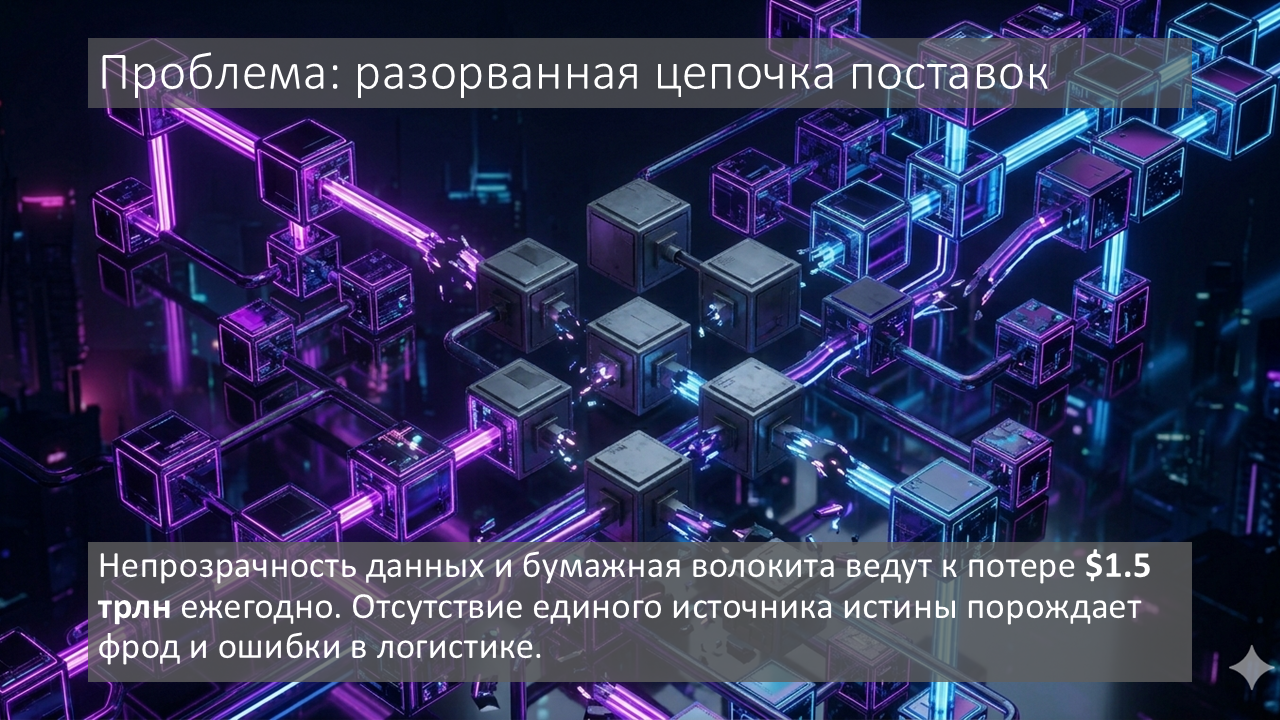
\includegraphics[width=17cm]{z4/s1.png}
	\caption{Слайд 1, модель (b)}
\end{figure}
\newpage
\begin{figure}[H]
	\centering
	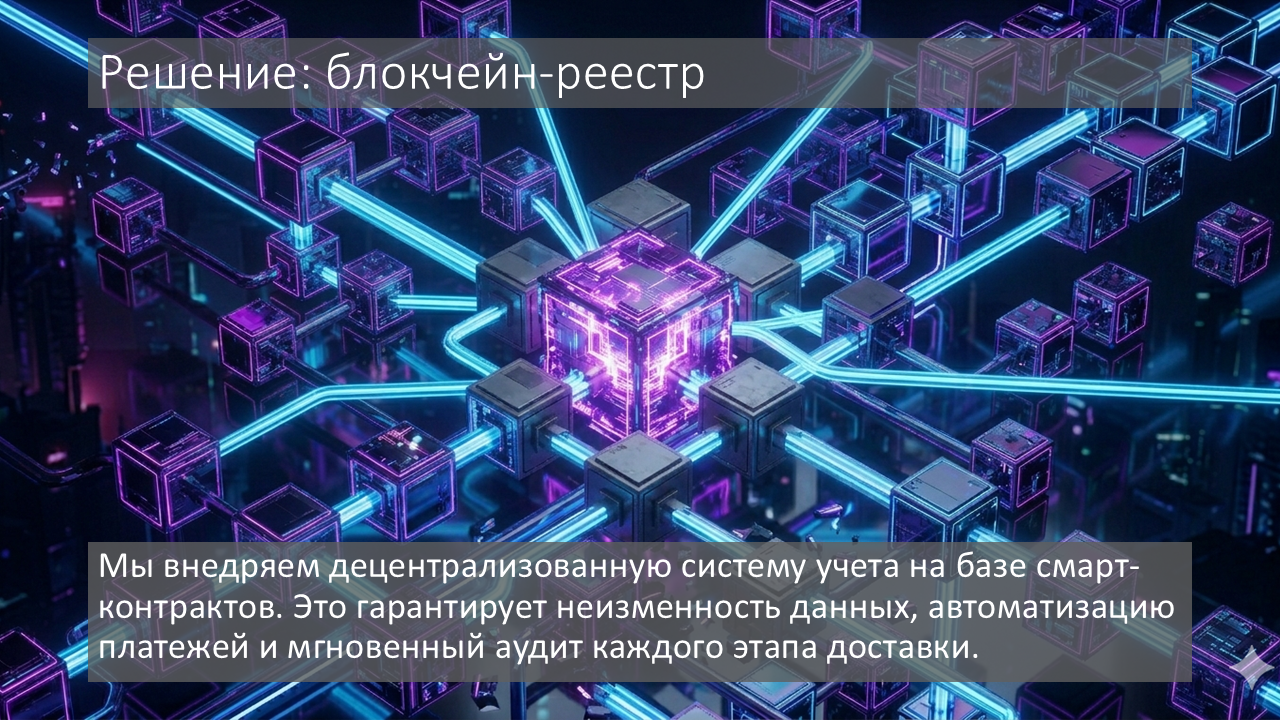
\includegraphics[width=17cm]{z4/s2.png}
	\caption{Слайд 2, модель (b)}
\end{figure}
% \newpage
\begin{figure}[H]
	\centering
	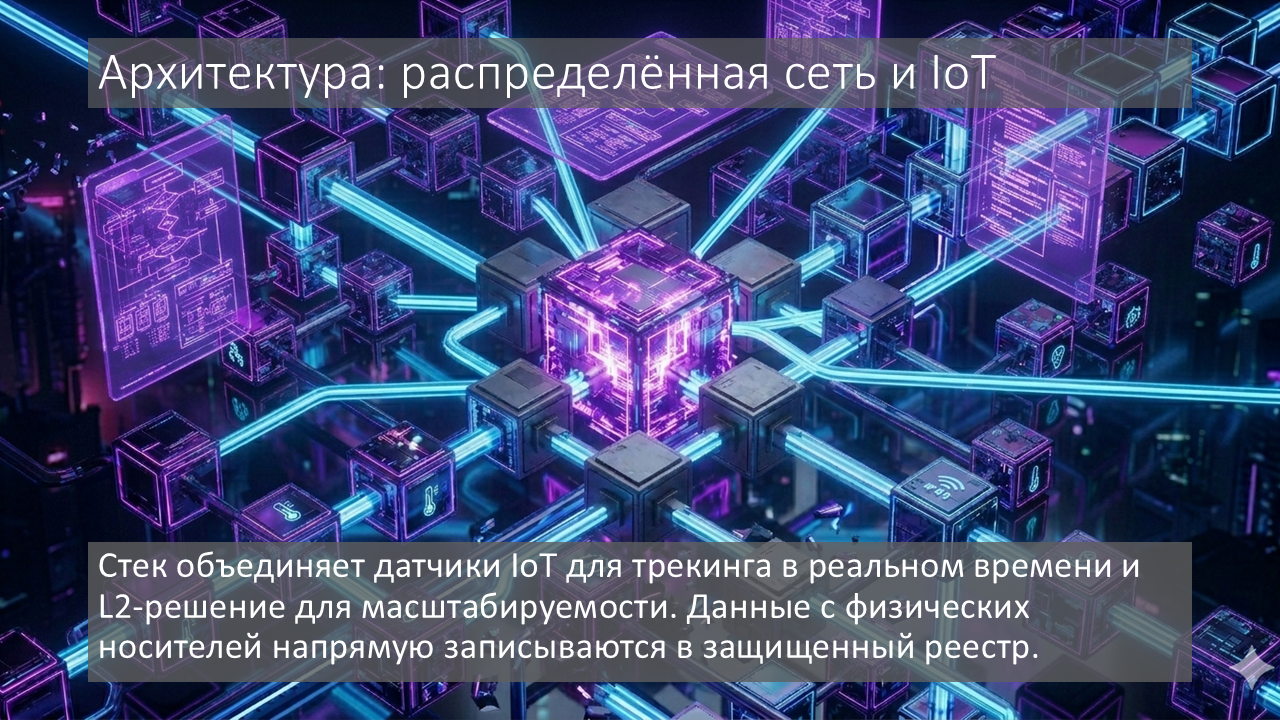
\includegraphics[width=17cm]{z4/s3.png}
	\caption{Слайд 3, модель (b)}
\end{figure}
\newpage
\begin{figure}[H]
	\centering
	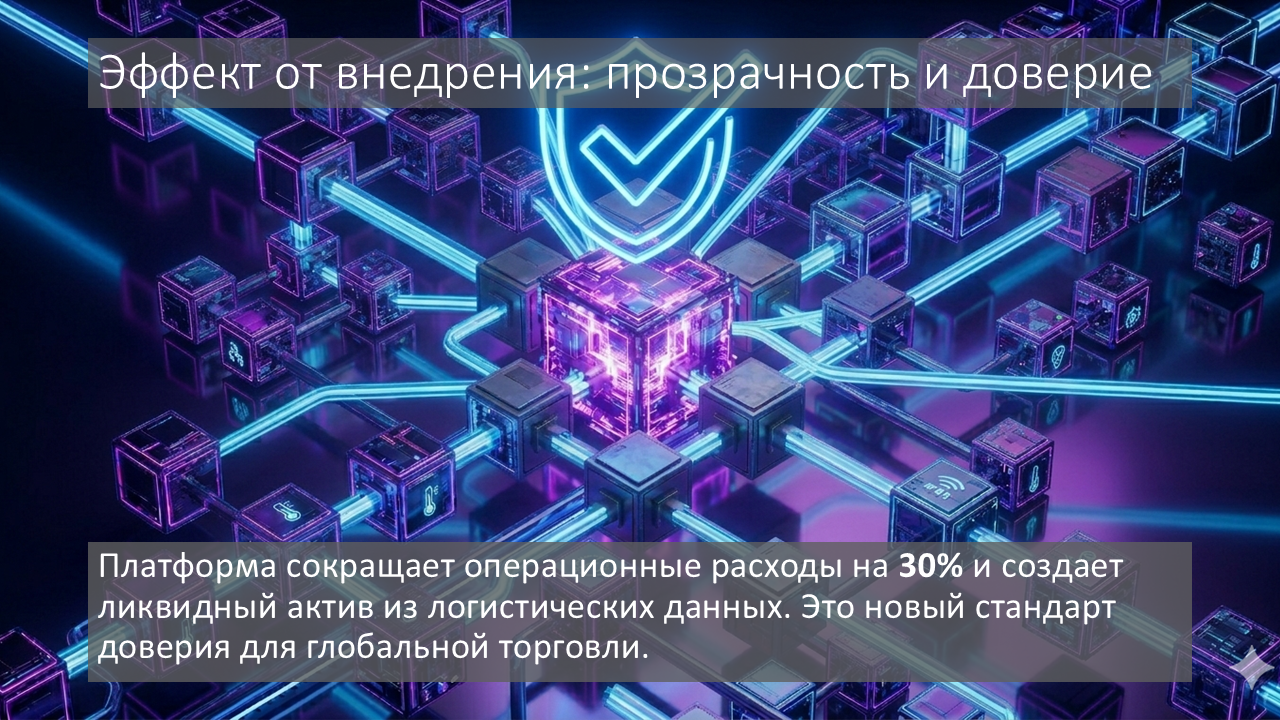
\includegraphics[width=17cm]{z4/s4.png}
	\caption{Слайд 4, модель (b)}
\end{figure}
Проверка согласованности: \\
Все четыре изображения выдержаны в единой цветовой гамме (чёрный, фиолетовый, голубой), используют одинаковые геометрические примитивы (кубы, линии), одинаковый тип освещения и угол обзора (изометрия). Различия только в сюжете и количестве объектов. Стилистическое единство достигнуто.
% \newpage
\subsection{Сравнение моделей}
\begin{table}[h!]
	\centering
	\begin{tabular}{|l|p{5cm}|p{5cm}|}
		\hline
		\textbf{Критерий} & \textbf{модель (a)} & \textbf{модель (b)} \\
		\hline
		Следование промпту & 3 & 5 \\
		\hline
		Качество деталей & 3 & 5 \\
		\hline
		Единство стиля на серии & 3 & 5 \\
		\hline
		Управляемость без Seed  & 3 & 5 \\
		\hline
		\textbf{Итог} & 3 & 5\\
		\hline
	\end{tabular}
\end{table}
\newpage
Модель (b) лучше подходит для задачи серийной генерации с единым стилем, когда недоступны ручные параметры (Seed, CFG). Модель (a) даёт более красивые одиночные кадры, но требует фиксации зерна для повторяемости, что не всегда удобно.
\subsection{Финальный промпт}
Итоговый шаблон промпта: \\
\textit{<<\{СЮЖЕТ\}, стиль: киберпанк, неон, тёмный фон, цветовая гамма – фиолетовый и голубой, изометрическая 3D-сцена, светящиеся кубы данных, соединённые толстыми линиями, без текста, без подписей, без лишних частиц, высокое разрешение, кинематографичное освещение, отражения на глянцевых гранях кубов>>} \\
\newline
Переменные части для четырёх слайдов:
\begin{enumerate}
	\item «Разорванная цепочка поставок в логистике: несколько потухших (серых) кубов и оборванные голубые линии между ними»
	\item «Блокчейн-реестр для логистики: центральный яркий фиолетовый куб, от которого отходят целые голубые линии ко множеству маленьких кубов по кругу»
	\item «Архитектура блокчейн-системы для логистики: множество кубов, соединённых в сеть, некоторые кубы имеют маленькие значки датчиков (IoT), сверху парят полупрозрачные схемы смарт-контрактов в виде светящихся фиолетовых скрижалей»
	\item «Результат внедрения блокчейн-реестра: все кубы ярко светятся фиолетовым и голубым, линии между ними целые и толстые, сверху над сценой появляется символ галочки или щита из голубого неона»
\end{enumerate}
\subsection{Вывод}
Для поддержания единого визуального стиля в текущей модели (и других закрытых моделях без доступа к Seed) эффективно использовать фиксированный суффикс стиля, одинаковый для всей серии. Ключевые слова, определяющие цветовую гамму, тип объектов, освещение и композицию, должны быть неизменны. Сюжетные вариации выносятся в начало промпта. Этот метод позволяет получить визуально согласованную серию изображений для презентации без необходимости вручную подбирать зерно.